\chapter{Modules}
\label{chap:Modules}

The source code of RespVis is structured into modules written in the ES module format.
Currently, all these modules are combined into a single, monolithic library bundle during the build process.
In the future, each module will be released on its own to allow users to import only the ones they need.
The reason for this is that most users will likely only require a subset of all the features included in the library and it would unnecessarily increase the size of their bundles to import all of them.
A good example of this is D3, which also separates its considerable amount of features into different modules that can be successively added to a project when the need arises.

At the time of writing, the RespVis library contains five different modules: the core, legend, tooltip, bar, and point modules.
Each of these modules contains submodules that have been grouped by thematic similarity.
The core module holds the core functionality of the library that all other modules depend on, which includes the layouter, axes, chart and chart window base components, and various utility functions and types.
The legend module contains the implementation of a legend component that is mostly meant to describe discrete data dimensions by rendering distinct values as labeled symbols.
The tooltip module holds functions to control the showing, placement, and content of tooltips, as well as utility functions that simplify the configuration and initialization of tooltips on series components.
% None of the modules listed so far contain components that render visual marks, which are characteristic for visualizations.
The bar module distinguishes between normal, grouped, and stacked bars and includes various low-level and high-level components to render each of those types.
Similarly, the point module contains low-level and high-level components to visualize point charts.
All of the different modules and the dependencies between them are shown in Figure~\ref{fig:Modules}. 

\begin{figure}[tp]
\centering
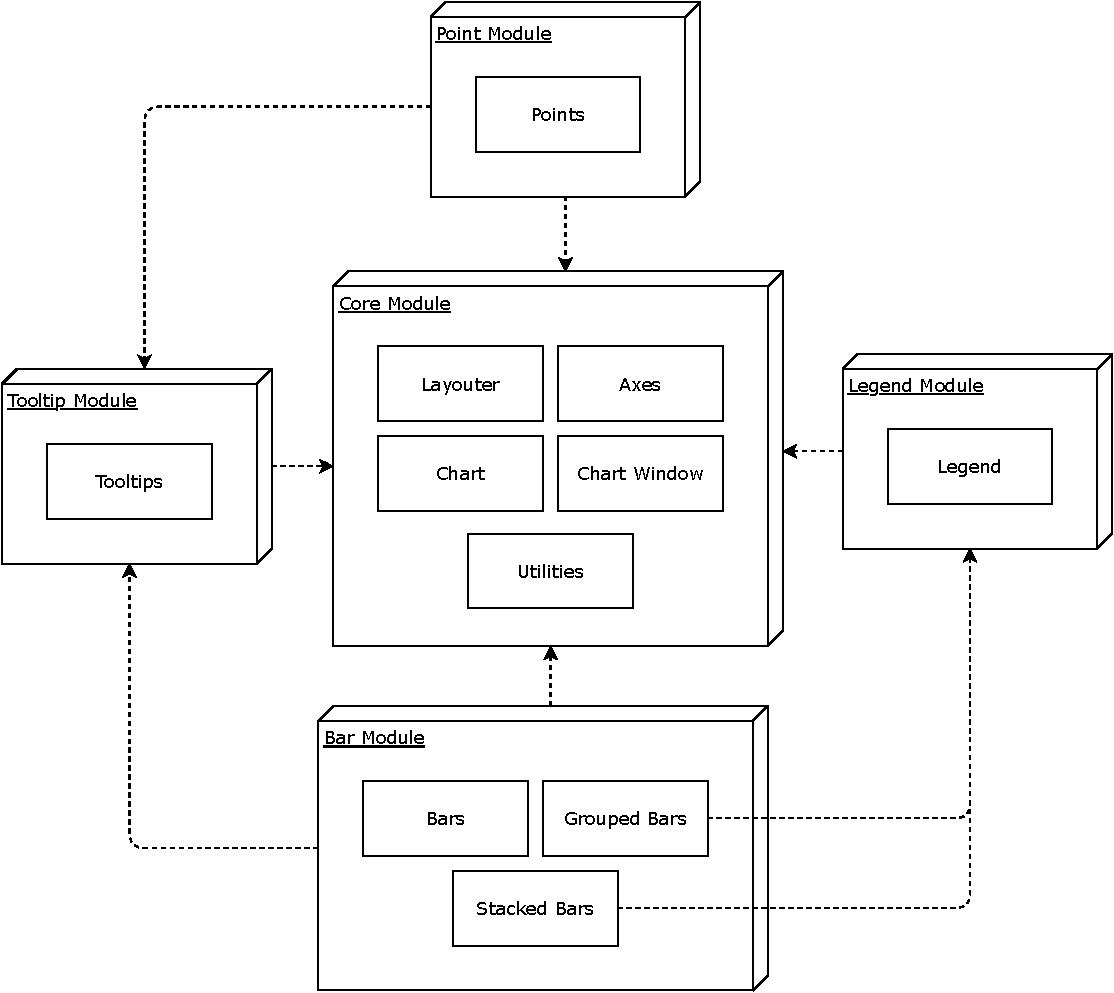
\includegraphics[keepaspectratio,width=\linewidth,height=\fullh]{diagrams/respvis-modules.pdf}
\caption[Modules of RespVis]{
  This diagram shows the different modules of the RespVis library.
  It also shows the most important submodules contained in the individual modules.
  The directional arrows connecting modules indicate dependencies between them. 
  \imgcredit{Image created by the author of this thesis using diagrams.net \TODO{Link properly}.}
}
\label{fig:Modules}
\end{figure}


\section{Core Module}

The core module contains the necessary core functionality of the library.
It is the base module that all other modules depend on and includes various utility functions, the layouter, axes, chart base components, and chart window base components.
RespVis heavily relies on utility functions to reuse and structure recurring operations.
The core module contains utilities to deal with arrays, elements, selections, and texts, as well as geometric utilities that simplify the handling of positions, sizes, rectangles, circles, and paths. 
The layouter is a custom component that enables controlling the layout of SVG elements with CSS.
% It achieves this by replicating the DOM tree of SVG elements that should be layed out with HTML \code{<div>} elements, applying the appropriate CSS configuration on the replicated elements, and storing their calculated layout information on the original SVG elements.
% Render functions can then use the stored layout information on layed out SVG elements to render their content so that it fits within the corresponding boundaries. 
Axis components have been included in the core module because they are important components that occur in nearly every visualization. 
% However, since only cartesian charts have been implemented thus far, only cartesian axes can be found in the implementation.
Lastly, the chart and chart window components provide base functionalities that simplify the creation of more specialized charts and chart windows.
The core module implementation is located in the \code{src/lib/core/} directory of the project.

\subsection{Utilities}

The utilities provided by RespVis are split on multiple modules that are placed in the \code{utilities/} directory of the core module.
These modules include types and functions that perform array, element, selection and text operations as well as modules that simplify geometric operations with positions, sizes, rectangles, circles and paths.
The naming of 


Array utilities can be found in the \code{utilities/array.ts} module.

The \code{utilities/elements.ts} module contains utilities that perform operations on elements. 

Selection utilities are implemented in the \code{utilities/selection.ts} module.
They include typing improvements for the D3 Selection, Transition and SelecionOrTransition interfaces and type guards to distinguish between Selections and Transitions.

Utilities for dealing with \code{<text>} elements can be found in the \code{utilities/text.ts} module.
It contains rather basic functionalities that simply set specific data attributes to specific values on \code{<text>} elements.
The text utility module holds functions that set data attributes controlling the horizontal and vertical alignment of \code{<text>} elements, as well as their orientation.
Horizontal and vertical alignment is configured using the \code{textAlignHorizontal} and \code{textAlignVertical} functions.
These functions respectively set the \code{data-align-h} and \code{data-align-v} attribute on a Selection or Transition to the value passed into either function as a string enum parameter of type \code{HorizontalAlignment} or \code{VerticalAlignment}.   
The \code{HorizontalAlignment} enum represents the string values \code{\"left\"}, \code{\"center\"} and \code{\"right\"}, while the \code{VerticalAlignment} enum represents the values \code{\"top\"}, \code{\"center\"} and \code{\"bottom\"}. 
The distinct \code{data-align-h} and \code{data-align-v} attribute values are then used in the \code{respvis.css} file to declare different \code{text-anchor} and \code{dominant-baseline} values that control the alignment of \code{<text>} elements. 
Text orientation is set using the \code{textOrientation} function.
This function sets the \code{data-orientation} attribute on a Selection or Transition to the value specified via the string enum parameter of type \code{Orientation}.
The \code{Orientation} enum represents the values \code{\"horizontal\"} and \code{\"vertical\"}.
These \code{data-orientation} values are then used in CSS to set a \code{<text>} elements \code{text-anchor}, \code{dominant-baseline}, and \code{transform} attributes, in order to rotate it accordingly and fit it into the bounding box of the 
Orientations other than these are currently not supported, but would be easy to implement by adding further values to the \code{Orientation} enum and providing additional CSS rules.



% array 
% elements
% selection
% text
% position
% size
% rect
% circle
% path

\subsection{Layouter}

% layouter

\subsection{Axes}

% base
% bottom axis
% left axis

\subsection{Chart}

% chart
% chart cartesian

\subsection{Chart Window}

% chart window
% menu dropdown
% series checkbox
% tool filter nominal
% tool download svg
% resize event dispatcher

\section{Legend Module}

\section{Tooltip Module}

\section{Bar Module}

\subsection{Basic Bars}

\subsection{Grouped Bars}

\subsection{Stacked Bars}

\section{Point Module}